\documentclass[resume]{subfiles}





\begin{document}
\begin{multicols}{3}
\section{Numérique}
\subsection{Circuits}
\paragraph{Combinatoires} Les sorties dépendent des entrées directement (porte logique par exemple)
\paragraph{Sequentiels synchrones} Les sorties dépendent de l'état actuel et des états précédents
\paragraph{Séquentiels asynchrones} Les sorties dépendent de l'état actuel, des états précédent et de l'état actuel des entrées et avec des délais non-contrôlés par l'horloge
\subsection{Comportement transitoire}
\paragraph{Rise time $t_r$} : Temps de montée de \SI{20}{\percent} à \SI{80}{\percent}
\paragraph{Fall time $t_f$} : Temps de descente de \SI{80}{\percent} à \SI{20}{\percent}
\paragraph{Edge rate} : $\frac{t_r+t_f}{2}$
\paragraph{Temps de contamination $t_{\cdelay}$ ($t_{\cdel}$)} : Temps le plus court avant qu'un changement sur l'entrée (\SI{50}{\percent}) apparaisse sur la sortie (\SI{50}{\percent})
\paragraph{Temps de propagation $t_{\pdelay}$  ($t_{\pdel}$)} : Temps le plus long avant qu'un changement sur l'entrée (\SI{50}{\percent}) apparaisse sur la sortie (\SI{50}{\percent})
\begin{figure}[H]
\centering
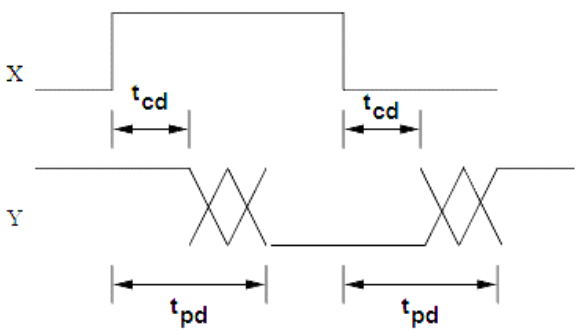
\includegraphics[width=4cm]{img_31.png}
\end{figure}
\paragraph{Temps de setup $t_{\text{setup}}$} : Temps de stabilité avant le flanc d'horloge
\paragraph{Temps de "hold" $t_{\text{hold}}$} : Temps de stabilité après le flanc d'horloge (souvent 0)
\begin{figure}[H]
\centering
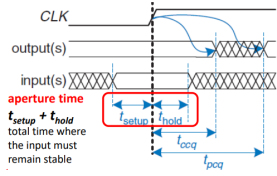
\includegraphics[width=4.00cm]{img_32.png}
\end{figure}
\subsection{Contraintes}
\subsubsection{Temps de setup}
\begin{figure}[H]
\centering
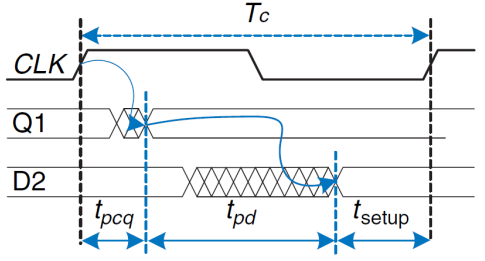
\includegraphics[width=4cm]{img_33.png}
\end{figure}
\begin{figure}[H]
\centering
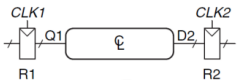
\includegraphics[width=3.00cm]{img_34.png}
\end{figure}
$$\boxed{T_{\text{clk}}\geq T_{\pdel cq}+t_{\pdelay}+t_{\text{setup}}\textcolor{darkgray}{+t_{\text{skew}}}}$$
Ou
$$\boxed{t_{\pdelay}\leq T_{\text{clk}}-(t_{\pdel cq} + t_{\text{setup}}\textcolor{darkgray}{+t_{\text{skew}}})}$$
\subsubsection{Temps de hold}
\begin{figure}[H]
\centering
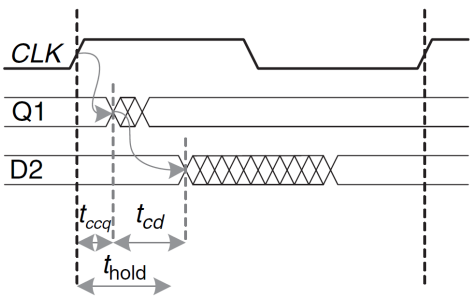
\includegraphics[width=4cm]{img_35.png}
\end{figure}
\begin{figure}[H]
\centering
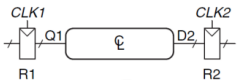
\includegraphics[width=3.00cm]{img_34.png}
\end{figure}
$$\boxed{t_{\cdel cq}+t_{\cdelay} \geq t_{\text{hold}}\textcolor{darkgray}{+t_{\text{skew}}}}$$
OU
$$\boxed{t_{\cdelay} \geq t_{\text{hold}}\textcolor{darkgray}{+t_{\text{skew}}}-t_{\cdel cq}}$$
\subsubsection{Circuit combinatoire}
\begin{figure}[H]
\centering
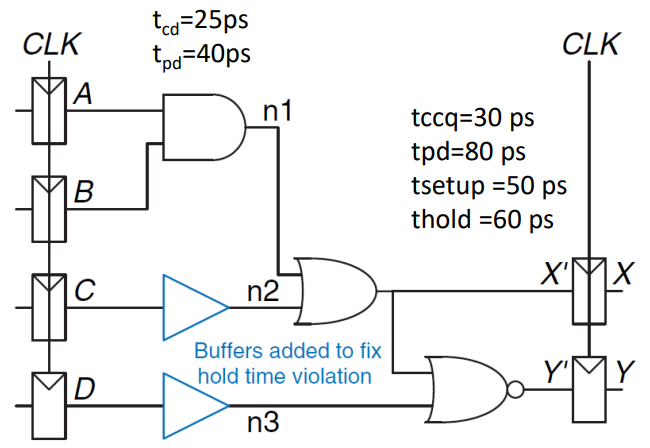
\includegraphics[width=6.00cm]{img_36.png}
\end{figure}
\subsection{Horloge}
\subsubsection{Skew}
Dans le cas des cascades de flip-flop
$$t_{\cdel cq} \geq t_{\text{skew}}$$
\subsection{FPGA}
\paragraph{Timing analysis} : Analyse des contraintes de timing du système complet et recherche des erreurs / définition de la fréquence max.\\
$t_{\pdelay}$ pour chaque logic element et $t_{\text{wire}}$ entre chaque logic element
\subsection{CMOS Transmission Gate}
\begin{figure}[H]
\centering
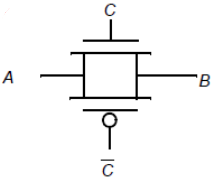
\includegraphics[width=4.00cm]{img_37.png}
\end{figure}
$C=1$ : Le système agis comme un fil.\\
$C=0$ : Le système agis comme un circuit ouvert
\subsection{Optimisation}
On va jouer sur : la micro-architecture, la logique, les circuits numériques, le layout (les deux derniers sont traités dans le cours)
\subsection{Capacités parasites}
\paragraph{Capacité de diffusion} : Capacité entre le drain et la sortie et entre source et sortie
\paragraph{Capacité de gate} : Capacité entre la gate et la masse (Canal N) et la gate et l'alimentation (canal P)
\subsection{Comportement transitoire d'un inverseur}
\begin{figure}[H]
\centering
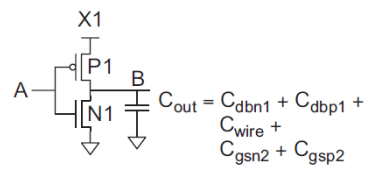
\includegraphics[width=5.00cm]{img_38.png}
\end{figure}
$$\frac{dV_B}{dt}=-\frac{\beta}{C_{out}}\begin{cases}\frac{(V_{DD}-V_{t})^2}{2} & V_B > V_{DD} - V_t\\
\left(V_{DD}-V_{t}-\frac{V_B}{2}\right)V_{B} & V_B<V_{DD}-V_t\end{cases}$$
\begin{figure}[H]
\centering
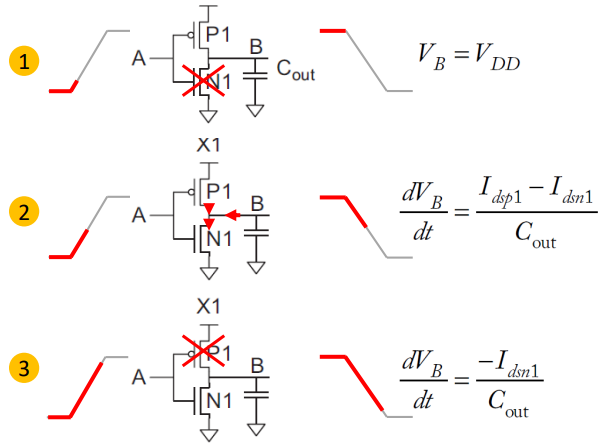
\includegraphics[width=\columnwidth]{img_39.png}
\end{figure}
\begin{enumerate}
\item $A$ commence à monter, $P_1$ est allumé $N_1$ est éteint et $B$ reste inactif
\item $A$ atteint $V_{tn}$, $P_1$ est allumé et $N_1$ s'allume ($B$ commence à diminuer)
\item $A$ est presque à $V_{DD}$, $P_1$ s'éteint et $B$ devient 0
\end{enumerate}
Si les temps de montée/descente en entrée ne sont pas 0, alors le temps de propagation augmente
\subsection{Modèle RC}
\begin{figure}[H]
\centering
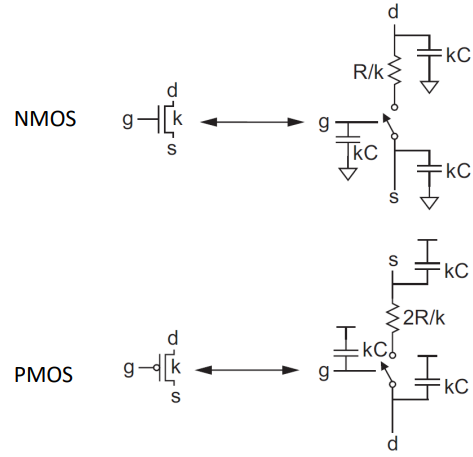
\includegraphics[width=\columnwidth]{img_40.png}
\end{figure}
$k$ est la "taille" du transistor (le nombre d'unités). Le Pmos a le double de résistance parce que les trous ont une moins bonne mobilité que les électrons. Pour avoir un circuit équilibré on utilise :
\begin{figure}[H]
\centering
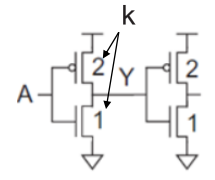
\includegraphics[width=3.5cm]{img_41.png}
\end{figure}
\subsubsection{Exemple de porte NAND à 3 entrées}
\begin{figure}[H]
\centering
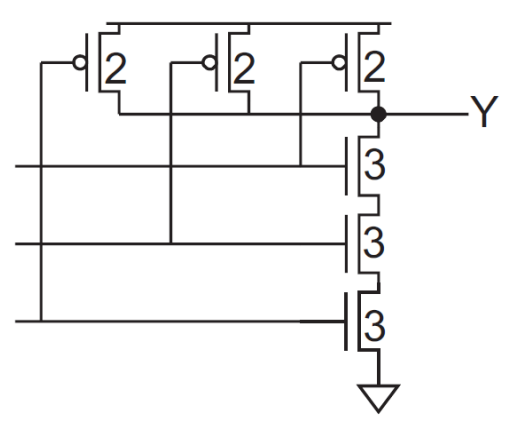
\includegraphics[width=5cm]{img_42.png}
\end{figure}
\begin{align*}
t_{\pdelay f}&=\ln(2)\cdot 12RC\\
t_{\pdelay r}&=\ln(2)\cdot 15RC\leftarrow\\
t_{\cdelay f}&=\ln(2)\cdot 9RC\\
t_{\cdelay r}&=\ln(2)\cdot 3RC\leftarrow
\end{align*}

\subsubsection{Exemple avec un inverseur}
$$V_{out}(t)=V_{DD}e^{-t/\tau}\qquad \tau=RC$$
$$\boxed{t_{\pdelay}=RC\ln(2)}$$
\subsection{Modèle de Elmore}
Un seul nœud d'entrée, tous les condensateurs sont entre des noeuds et le GND, aucune boucle résistive
\begin{figure}[H]
\centering
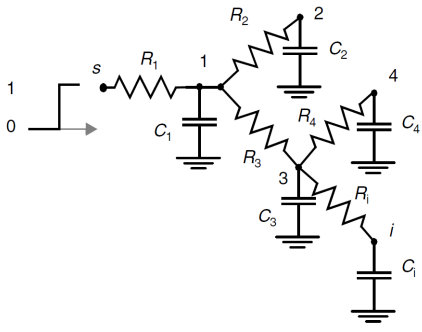
\includegraphics[width=5.00cm]{img_43.png}
\end{figure}
Délai sur le nœud $i$ :
\begin{align*}
\tau_{Di}&=R_1C_1\\&+(R_1\textcolor{OrangeRed}{+R_2})C_2\\&+(R_1+R_3)C_3\\&+(R_1+R_3\textcolor{OrangeRed}{+R_4})C_4\\&+(R_1+R_3+R_i)C_i
\end{align*}
\textcolor{OrangeRed}{Vérifier ce qui est en rouge !}
\subsubsection{Représentation linéaire}
$$\frac{\tau_{\pdelay}}{\tau}=d=(p+f)$$
\paragraph{Délai parasite $p$} : Propre à la porte logique (en principe invariant)
\paragraph{Délai "d'effort" $f$} : Dépend des charges
\paragraph{Effort électrique $h$} : Rapport entre la capacité d'entrée et de sortie $C_{out} / C_{in}$

\begin{figure}[H]
\centering
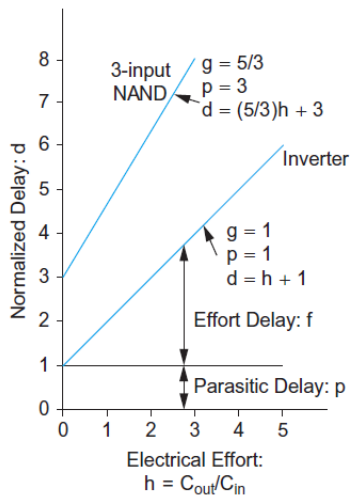
\includegraphics[width=4.00cm]{img_44.png}
\end{figure}
\subsubsection{Délais parasites}
\begin{figure}[H]
\centering
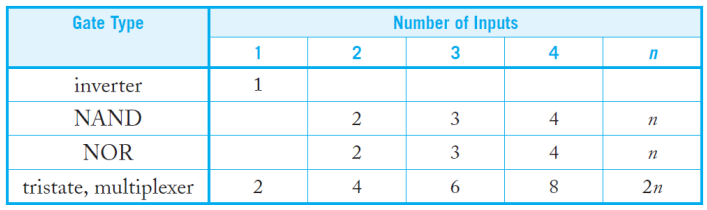
\includegraphics[width=0.9\columnwidth]{img_46.png}
\end{figure}
\subsubsection{Efforts logiques}
\begin{figure}[H]
\centering
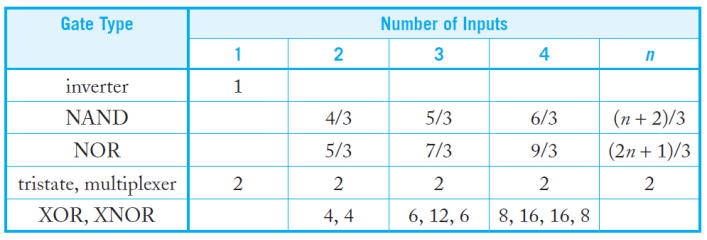
\includegraphics[width=0.9\columnwidth]{img_47.png}
\end{figure}
Des portes avec moins d'entrées sont mieux que des portes avec plus d'entrées
\subsection{Système à plusieurs étages}
\paragraph{effort logique du chemin $G$}
$$G=\prod g_i$$
\paragraph{Effort électrique du chemin $H$}
$$H=\frac{C_{out(\text{path})}}{C_{in(\text{path})}}$$
\paragraph{Effort du chemin $F$}
$$F=\prod f_i=\prod g_ih_i$$
$$F\neq GH\quad (\text{avec plusieurs chemins})$$
$$\boxed{F=GBH}$$
\paragraph{Effort "d'embranchement" $B$}
$$b=\frac{C_{\text{sur le chemin}}+C_{\text{hors chemin}}}{C_{\text{sur le chemin}}}$$
$$B=\prod b_i$$
\begin{figure}[H]
\centering
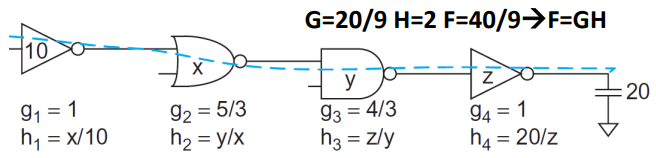
\includegraphics[width=\columnwidth]{img_48.png}
\end{figure}

\begin{figure}[H]
\centering
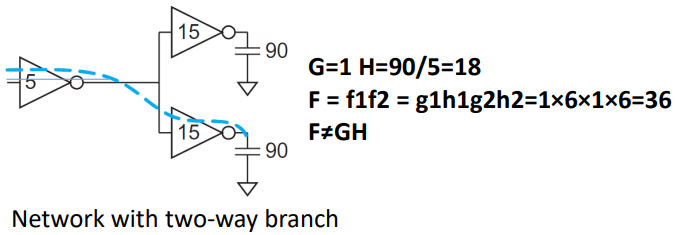
\includegraphics[width=\columnwidth]{img_49.png}
\end{figure}
\paragraph{Délai du chemin $D$}
$$D=\sum d_i=D_F+P$$
\paragraph{Délai d'effort du chemin $D_F$}
$$D_F=\sum f_i$$
\paragraph{Délai parasite $P$}
$$P=\sum p_i$$
\subsubsection{Autres}
Effort pour chaque étage ($N$ étages)
$$\hat{f}=g_ih_i=F^{1/N}$$
Délai minimal pour $N$ étages avec effort $F$ et délai parasite $P$
$$D=NF^{1/N}+P$$
\begin{figure}[H]
\centering
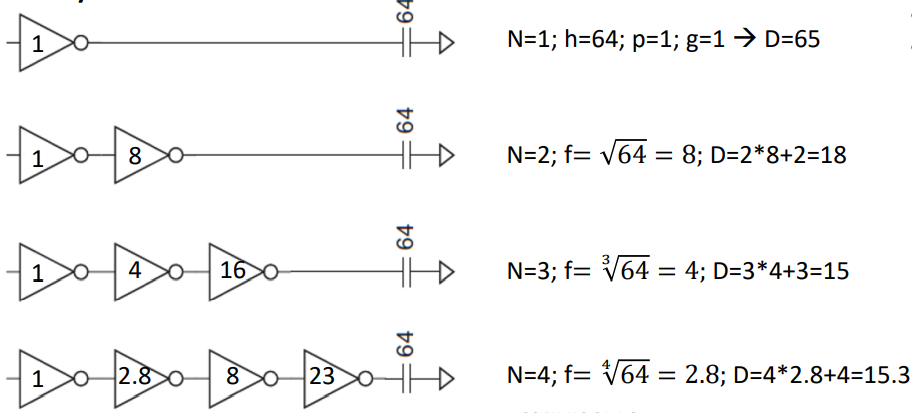
\includegraphics[width=\columnwidth]{img_50.png}
\end{figure}
\end{multicols}
\begin{figure}[H]
\centering
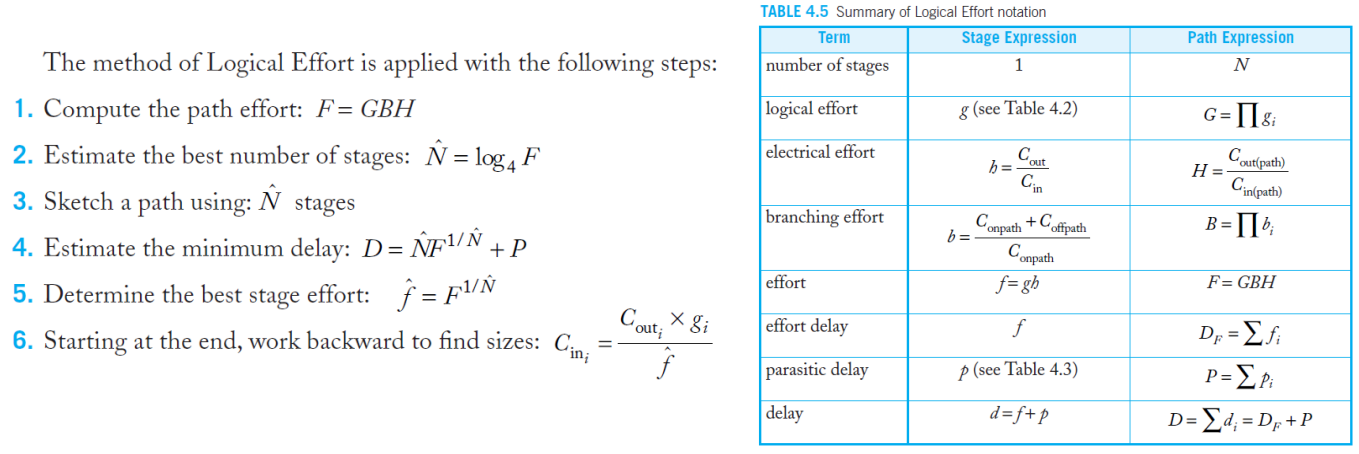
\includegraphics[width=16.00cm]{img_51.png}
\end{figure}
\end{document}